\section{需求}
\subsection{功能需求}
\label{c31}
地面站软件系统功能如图\ref{f3fun}所示。
\begin{figure}[ht]
	\begin{center}
		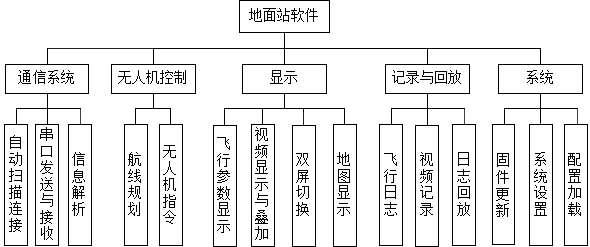
\includegraphics{function.png}
		\caption{地面站系统功能结构图}
		\label{f3fun}
	\end{center}
\end{figure}

\subsubsection{自动扫描连接}
地面站系统只会同时与一台无人机建立连接。

当连接正常接入时,软件能够自动识别连接使用的串口,接入的硬件和使用的通讯协议,并在10s内与飞控建立连接。
连接建立后忽略所有新出现的串口连接。软件通过检测心跳包判断连接是否可用,当一定时间没有接收到心跳包后认为连接断开。心跳包丢失时间可在软件中进行设置。

在建立连接前,若存在无法识别通信协议的串口连接,软件将使用串口通信设置的波特率持续对串口进行扫描,直到出现可识别的串口。

\subsubsection{串口发送与接收}
地面站系统使用串口通过直接连接或经由数传电台与无人机飞控进行通信。
串口通信波特率为115200,可以通过地面站设置更改串口使用的波特率。

当串口意外断开时,软件能够捕获异常并做适当处理,保证运行的稳定。

\subsubsection{信息解析}
地面站系统接收到数据包后,根据通信协议解析接收缓存并提取数据包,供其他功能模块使用,或接受其他功能模块传递的数据包,将其转换为数据流经由串口发送。

\subsubsection{任务航线规划}
地面站系统能够进行任务航线规划,任务由一系列按顺序相连的任务项组成。使用的任务项如表\ref{t3miss}所示。
任务项通过点击地图或输入参数设置,或通过子任务加载或自动生成。任务航线可以保存到本地文件,或从文件中读取。

任务规划完毕后通过串口通信发送至无人机飞控,飞控不支持的任务项类型将被自动忽略。

\begin{table}[ht]
\centering
\caption{任务项}
\label{t3miss}
\begin{tabular}{|l|l|}
\hline
\multicolumn{1}{|c|}{类别} & \multicolumn{1}{c|}{任务项} \\ \hline
航路点                      & 初始点,导航点,起降点,环绕点          \\ \hline
动作                       & 拍照,投放载荷,模态转换,操作任务载荷      \\ \hline
子任务                       & 子任务,扫描区域                 \\ \hline
飞行控制                     & 改变速度,改变高度                \\ \hline
\end{tabular}
\end{table}

\subsubsection{无人机指令}
地面站系统能够直接向无人机飞控发送指令,指示飞控完成一定的动作。发送的指令主要包括以下几类:
\begin{itemize}
\setlength{\itemsep}{-2pt}
\item 飞行指令:控制无人机飞行的指令,包括起飞,降落,返航,飞行模式切换,飞行到目标点等。
\item 飞控指令:命令飞控执行动作,包括校准传感器,锁定或解锁飞控,获取和设置飞控参数等。
\item 任务指令:与任务相关的指令,包括发送和接收任务或单独的任务项,开始或终止任务等。
\end{itemize}

指令发送后由地面站判定是否发送成功,若发送失败将自动重发若干次,重发次数可由用户设定。


\subsubsection{飞行参数显示}
地面站系统通过通信系统获取飞行数据,并以一定的方式将其中的部分参数显示在软件界面中。界面中直接显示的数据见表\ref{t3dppara}。
所有数值全部使用SI单位。

对于不同的飞控硬件,发回的数据内容可能并不相同。若飞控没有发送需要显示的参数,地面站中将显示参数的缺省值。
若飞控中途断开连接,软件将保持显示最后一次接收到的数值。

\begin{table}[ht]
\centering
\caption{显示的飞行参数}
\label{t3dppara}
\begin{tabular}{|l|l|}
\hline
\multicolumn{1}{|c|}{参数类型} & \multicolumn{1}{c|}{参数名}  \\ \hline
飞行姿态 & 俯仰角,滚转角,机头指向              \\ \hline
飞行状态 & 空速,地速,航向,上升/下降率,相对高度,飞行模式 \\ \hline
定位状态 & 精度,纬度,卫星数,定位状态,定位误差       \\ \hline
导航状态 & 航程,航时,回航角,航点信息            \\ \hline
动力状态 & 电池电压,电池电流,估计剩余电量          \\ \hline
通信状态 & 通信速率,通信协议,RSSI            \\ \hline
\end{tabular}
\end{table}

\subsubsection{视频显示与叠加}
地面站系统能够显示视频画面,同时在画面中叠加部分飞行参数和图形提示。

在无人机飞行时,视频画面由图传电台接收,通过视频采集卡获取视频流进行显示;
在回放时,视频从本机硬盘中读取。

\subsubsection{双屏切换}
地面站系统能够拆分为两个窗口,分别显示于两个显示器中。
其中一个窗口显示地图和飞行参数,另一个窗口显示机载摄像设备传回的画面。
在运行过程中两个显示器中的窗口可以快速交换位置。

若无视频流传入,则摄像画面窗口显示空白内容。

\subsubsection{地图显示}
地面站系统能够显示普通地图,卫星地图或混合地图,并能够在三种地图之间切换。
除地图外,还能够在地图上实时显示无人机位置,方向,飞行轨迹和预设航线。

地图使用国内电子地图平台,能够预先缓存指定地区的离线地图,地图上显示误差不超过0.1m。

\subsubsection{飞行日志}
地面站系统通过通信系统接收到合法的数据包后,将数据包连同时间戳作为飞行日志储存于本地硬盘中,以便回放使用。
飞行日志实时写入硬盘临时文件中,当用户选择停止写入或关闭地面站时,将弹出保存窗口用以指定日志文件保存位置。
若飞行过程中地面站意外关闭,临时文件没有损坏,则可以通过临时文件恢复意外关闭前的飞行记录。

\subsubsection{视频记录}
地面站系统接收到图传电台传回的视频数据流,将视频原始数据流以视频文件的格式储存在本地硬盘中,同时记录视频时间与飞控运行时间的相对关系。

若飞行过程中地面站意外关闭,视频记录文件将部分损坏。

\subsubsection{日志回放}
地面站系统能够读取飞行日志和视频记录,并进行回放。
回放时可以单独回放飞行日志,或同时回放飞行日志和视频画面。
回放速度和进度均可以手动实时调节。

当同时回放视频与日志时,飞行参数仍以与飞行时相同的方式叠加在视频上。


\subsubsection{固件更新}
地面站系统能够对飞控固件进行更新和烧写。

\subsubsection{系统设置}
对地面站软件中的部分参数进行设置,并可将设置信息以配置文件的形式保存至文件。

\subsubsection{配置加载}
地面站系统可从外部文件加载配置信息,以快速适配不同的无人机系统或使用环境。

若加载的配置文件与地面站版本不同,加载中将忽略地面站软件不存在配置参数,同时保持文件中没有指明的参数不变。

\subsection{外部接口需求}

\subsubsection{接口标识和接口图}
地面站系统外部接口如图\ref{f3int}所示。接口简述如表\ref{t3int}所示。
\begin{figure}[ht]
	\begin{center}
		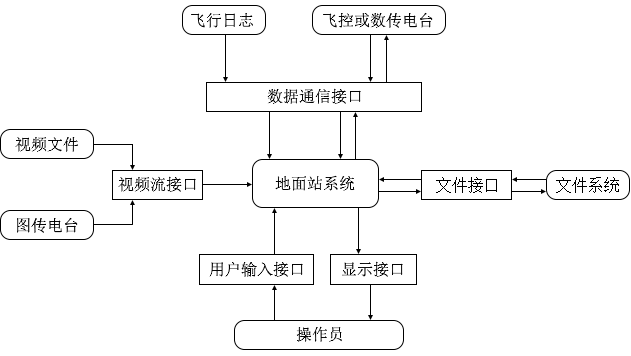
\includegraphics{interface.png}
		\caption{外部接口图}
		\label{f3int}
	\end{center}
\end{figure}

\begin{table}[ht]
\centering
\caption{外部接口说明}
\label{t3int}
\begin{tabular}{|l|l|}
\hline
\multicolumn{1}{|c|}{接口名称} & \multicolumn{1}{c|}{接口简述}    \\ \hline
数据通信接口                     & 使用特定的通讯协议,用于与飞控进行通信,或读取日志文件用于回放 \\ \hline
视频流接口                      & 用于从外部获取视频数据                  \\ \hline
文件接口                       & 用于向磁盘中写入飞行日志和视频记录,写入或读取配置信息  \\ \hline
用户输入接口                     & 用于获取操作员对地面站系统的输入             \\ \hline
显示接口                       & 用于在显示器中绘制图形界面                \\ \hline
\end{tabular}
\end{table}
\subsection{计算机资源需求}
\subsubsection{计算机硬件需求}
运行地面站软件的计算机硬件需求配置如表\ref{t3req}所示。

\begin{table}[ht]
\centering
\caption{计算机硬件需求}
\label{t3req}
\begin{tabular}{|l|l|}
\hline
\multicolumn{1}{|c|}{硬件} & \multicolumn{1}{c|}{最低需求} \\ \hline
处理器                      & Intel Core i5             \\ \hline
内存                       & 4G 双通道                       \\ \hline
图形                       & Intel HD530               \\ \hline
储存空间                     & 1G SSD                    \\ \hline
显示                       & 每个显示器实际分辨率1366*768        \\ \hline
\multirow{2}{*}{其他}      & 至少一个USB接口                 \\ \cline{2-2} 
                         & 支持DirectShow的视频采集卡        \\ \hline
\end{tabular}
\end{table}

其中储存空间需求为保证地面站正常运行和记录日志的最低要求,不包含储存飞行视频的空间需求。

\clearpage
\subsubsection{计算机软件需求}
\begin{itemize}[topsep=0pt]
\setlength{\itemsep}{-2pt}
\item Windows 7及以上的Windows操作系统
\item Microsoft .NET Framework 4.5
\item Microsoft .NET Framework 4.0
\item Microsoft DirectX 9.0c 及以上
\item 用于连接数传电台和飞控的串口驱动程序
\item 视频采集相关驱动程序
\end{itemize}

\endinput